\section{External validity: published instances, a longer horizon, offline knowledge and a second domain}
\label{sec:external}
The synthetic classes are the weakest point of any such study because the authors chose them. We therefore repeated the protocol on instances that others defined, and then asked how far the conclusions carry.

\subsection{Published families and the standard benchmark}
\label{sec:families}\label{sec:fanjul}
On three published families of $R||\Cmax$ ($500$ test instances per family and space; learners with frozen hyperparameters, only the validated action re-chosen) the cross-fitted headroom exceeds the threshold in all six cells ($0.52$ to $2.31$ points) and the validated action beats every learner in all $30$ pairs ($0.42$--$2.64$ points). But the standard Q-Learning gains beyond the margin in four of the six cells, up to $0.67$ and $0.83$ points with correlated machines ($53\%$ and $65\%$ of the validated gain). We first read this as the most favourable evidence for online learning that we found, and withdraw that reading in Section~\ref{sec:order}: an order-invariant Q-Learning loses to random choice in all six cells. An irace-configured static action is at parity with the validated one in every cell; an irace-tuned Q-Learning and two published designs gain up to $0.82$ and $0.54$ points, and the validated action beats the three in all $18$ comparisons.

On the standard benchmark ($28$ classes of type and $n$, the validated action chosen on $10$ tuning instances per class, learners frozen) the validated action gains beyond the margin in all $21$ cells ($0.14$ to $5.08$ points) and is better than every learner in all $147$ learner--cell pairs; its mean gap to the best known solutions of the $700$ test instances is $4.89\%$ in the richest space (B30), against $7.42\%$ for random choice. The standard Q-Learning gains in three of its $21$ cells, loses up to $1.19$ points, and does worst where the static choice matters most; the diagnostic of Section~\ref{sec:order} explains why: it puts $55\%$ of its choices on the first, cheapest action. Five of the seven registered predictions held.

\subsection{Equal CPU time, a longer horizon and a neural policy}
\label{sec:eqcpu}\label{sec:longT}\label{sec:neural}
\emph{Equal CPU time.} Measured $K$ is $0.74$ for the standard Q-Learning, $0.98$--$1.07$ for most learners and $1.97$ for the validated action, which therefore runs about half as many iterations. The standard Q-Learning's cost effect is $+0.44$ points, so at equal CPU it is level with random choice ($-0.03$; at equal iterations $-0.46$) and wins beyond the margin in two of seven types, those where the cheapest action it repeats happens to be good. The validated action, with half the iterations, still beats the learners in $44$ of the $49$ learner--type pairs; two pairs go the other way (an outcome we had predicted not to happen), on correlated machines, where the local-search action is the most expensive (median $K=2.50$): the ALNS roulette and the FRRMAB-style design beat it by $0.29$ and $0.53$ points.

\emph{A ten times longer horizon.} At $T=10{,}000$ the validated action is $2.69\%$ above the best known solutions ($4.89\%$ at $T=1000$) and its gain over random choice falls from $2.26$ to $1.50$ points; it again beats all $49$ learner--type pairs, and the best learner of each type recovers from $12\%$ to $39\%$ of its gain. The order-invariant Q-Learning gains beyond the margin in none of the seven types and is worse than random choice in six.

\emph{A neural policy trained offline.} A network with one hidden layer, trained by evolution strategies~\cite{SalimansEtal2017} on the $280$ tuning instances to map the state of the search and the instance features to a softmax over the actions (frozen at test time; training cost not charged to it), gains beyond the margin in all $14$ cells and more than the best of seven online learners in all $14$, but never beats the validated action. Averaged over the $14$ cells the validated action gains $1.95$ points, the policy $1.31$ ($67\%$), a constant mixture of actions trained with the same budget $1.17$ ($60\%$) and the best online learner of each cell $0.35$ ($18\%$): knowledge acquired before the run is worth about $3.7$ times what the best online learner finds during it, and most of its value is a good mixture, not a state-dependent decision.

\subsection{How much offline knowledge does a static action need, and can the online learner use it?}
\label{sec:granularity}
\paragraph{Design} We ran all $30$ fixed actions of B30 on the $700$ test instances and evaluated static policies chosen \emph{only on the tuning instances} with decreasing knowledge: one action for all instances ($G_0$), one per type ($G_t$), per size ($G_n$) and per class ($G_{tn}$, the validated action); two transfer regimes withhold the tuning data of the tested type or size. The nine predictions and the hashes were recorded before the actions were run on the test instances.

\paragraph{Results} Figure~\ref{fig:granularity} and Table~\ref{tab:granularity} give the gains. With no knowledge of the instance, one action gains $1.15$ points in B30, $51\%$ of the class-validated gain ($2.24$), and beats random choice beyond the margin in six of seven types; the best online learner of each type gains $0.39$ ($17\%$), and none of the seven learners beats $G_0$ in any of the $49$ pairs. The size of the instance carries most of the knowledge: $G_n$ recovers $89\%$ of the class-validated gain ($2.00$), whereas the type adds nothing over $G_0$ ($G_t$: $1.19$). A static action transfers to an unseen \emph{type} ($G_0$ without the type still gains $1.00$) but not to an unseen \emph{size}: $G_0$ and $G_t$ chosen without the tested size gain $0.34$ and $0.38$ points ($15\%$ and $17\%$). The neural policy, which receives $\ln n$ and $\ln m$, gains $1.55$ points ($69\%$). Seven of the nine predictions held.

\begin{figure}[t]
\centering
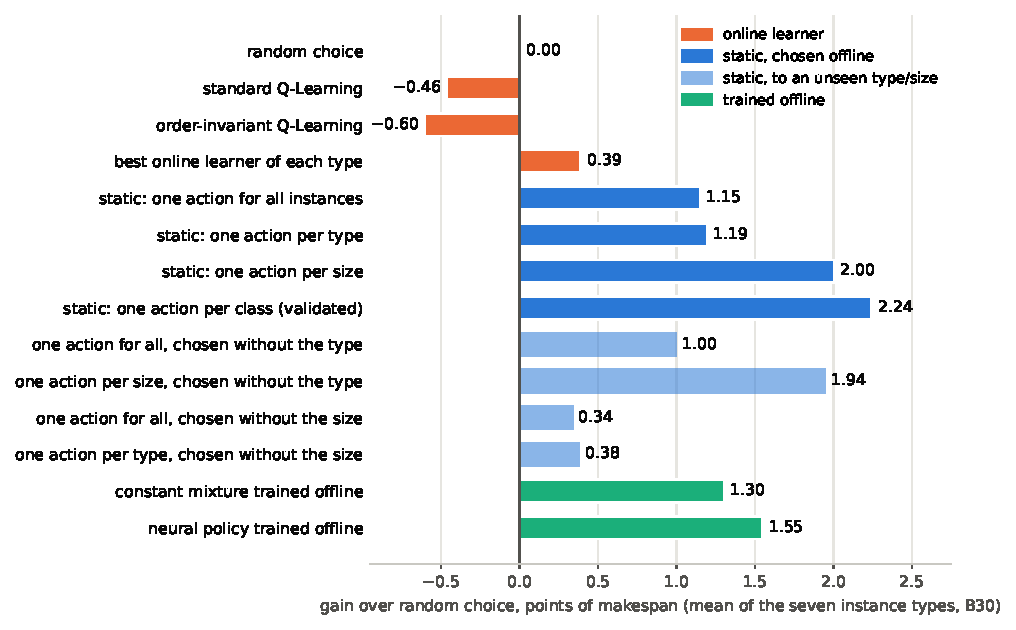
\includegraphics[width=0.92\textwidth]{fig_granularity.pdf}
\caption{The value of offline knowledge by granularity (standard benchmark, B30): gain over random choice, mean of the seven instance types. Orange: online learners; blue: static actions chosen on the tuning instances (hatched: chosen without the type or the size of the instances tested); green: policies trained offline; dotted orange: the optimistic Q-Learning warm-started with an offline prior (and, in blue, the same prior without learning).}
\label{fig:granularity}
\end{figure}

% Auto-generated by analysis/make_table_journal.py
\begin{table}[t]
\caption{The value of offline knowledge by granularity on the standard benchmark: gain over random choice (points of makespan; mean of the seven instance types, $100$ test instances each, $T=1000$, three seeds) of static actions chosen on the tuning instances with decreasing knowledge of the instance, of the online learners and of the policies trained offline. B30 also shows the share of the class-validated gain. Static actions are chosen only on the tuning instances; the ceiling chooses on two test seeds and evaluates on the third.}
\label{tab:granularity}
\centering
{\scriptsize\setlength{\tabcolsep}{5pt}
\begin{tabular}{@{}lrrrr@{}}
\toprule
Policy & B5 & B15 & B30 & B30, share of $G_{tn}$ \\
\midrule
random choice & 0 & 0 & 0 & 0 \\
best online learner of each type & 0.22 & 0.31 & 0.39 & 17\% \\
standard Q-Learning & $-$0.33 & 0.05 & $-$0.46 & $-$21\% \\
order-invariant Q-Learning & $-$0.06 & $-$0.24 & $-$0.60 & $-$27\% \\
static, one action for all instances ($G_0$) & 0.28 & 1.02 & 1.15 & 51\% \\
static, by type ($G_t$) & 0.32 & 0.99 & 1.19 & 53\% \\
static, by size ($G_n$) & 0.57 & 1.30 & 2.00 & 89\% \\
static, by class (type, size): the validated action ($G_{tn}$) & 0.87 & 1.60 & 2.24 & 100\% \\
static, by class, chosen on the test seeds (cross-fitted ceiling) & 0.87 & 1.61 & 2.23 & 99\% \\
$G_0$ chosen without the type of the instance & 0.28 & 1.02 & 1.00 & 45\% \\
$G_n$ chosen without the type of the instance & 0.35 & 1.10 & 1.94 & 87\% \\
$G_0$ chosen without the size of the instance & 0.28 & 1.02 & 0.34 & 15\% \\
$G_t$ chosen without the size of the instance & $-$0.40 & 0.33 & 0.38 & 17\% \\
constant mixture trained offline (nn\_const) & -- & 1.03 & 1.30 & 58\% \\
neural policy trained offline (nn) & -- & 1.07 & 1.55 & 69\% \\
\bottomrule
\end{tabular}}
\end{table}


\paragraph{Where online learning pays, and how to build it (post hoc, then registered)} The unseen-size regime is the one place where an online learner beat an offline static action, at the two extreme sizes ($n=100$ and $n=1000$): at $n=100$ the transferred action \emph{loses} $1.19$ points to random choice while the FRRMAB-style learner is level with it, and at $n=1000$ the optimistic Q-Learning gains $0.83$ against $0.37$. We then built the insurance: the optimistic Q-Learning is warm-started with a prior computed on the tuning instances only (the initial value of an action is its score in $[0,1]$ times the optimism factor of the cold learner). With the prior taken from the other sizes it gains $1.07$ points, against $0.31$ for the cold learner and $0.38$ for the transferred static action. With the prior of the class itself it gains $1.97$ ($88\%$ of the class-validated gain) but never beats the class-validated action. A control with the learning rate set to zero shows what learning adds: without it the transferred prior is worth what the transferred static action is worth ($0.40$ against $0.38$) and the class prior what the validated action is worth ($2.25$ against $2.24$); learning adds $0.67$ points when the prior was transferred (six of seven types) and costs $0.28$ when the prior was exact. The online learner is a \emph{corrector} of offline knowledge: it earns what the prior lacks and pays for what the prior already had. Six of the seven predictions of the warm-start battery held, and all five of its control.

\subsection{A second domain: the iterated local search for the travelling salesman problem}
\label{sec:tsp}
\paragraph{Design and results} To test whether the findings belong to scheduling, we applied the protocol unchanged to an iterated local search for the Euclidean TSP: a tour improved by 2-opt and Or-opt with neighbour lists, a perturbation chosen at each iteration by the selector (a local double-bridge, short random reversals, or the shuffle of a segment; five sizes of each; spaces T5 and T15) and acceptance of a candidate that is not worse. Instances are uniform or clustered points with $n\in\{200,500,1000,2000\}$ (eight classes, $12$ tuning and $50$ test instances each, $T=1000$, three seeds; learners with frozen hyperparameters). The picture of the scheduling hosts repeats (Table~\ref{tab:tsp}). The validated action gains over random choice beyond the margin in all $16$ cells ($0.05$ to $0.90$ points of the tour length) and none of the six online learners beats it beyond the margin in any of the $96$ learner--cell pairs. The standard Q-Learning loses to random choice in every cell ($0.13$ to $0.63$ points) and the lock-in reproduces: it puts $61\%$ of its choices in T15 on the action listed first and evaluates $0.64$ times as many moves as random choice; the permuted version gains in no cell and differs from it beyond the margin in $15$ of $16$ cells. Thompson sampling gains in $7$ of $16$ cells (up to $0.38$ points), but the best online learner of a cell recovers at most half of the validated gain in $12$ of the $16$. All ten predictions held. On $37$ instances of the TSPLIB~\cite{Reinelt1991} (static actions chosen only on the synthetic tuning instances), the static action gains beyond the margin in both spaces ($0.53$ and $0.56$ points; one action for all gains $0.53$ and $0.68$), no online learner beats it, the best, Thompson sampling, recovers $23\%$ and $43\%$ of its gain, and the static action ends on average $1.21\%$ above the optimal tour in T15 (random choice: $1.79\%$); all nine predictions held.

\paragraph{The hierarchy of knowledge is not universal} In the TSP the finest knowledge adds nothing: one action chosen for all instances gains $0.54$ points in T15, more than the class-validated action ($0.50$, chosen on $12$ tuning instances per class), and the action chosen without the size of the tested instances gains beyond the margin at all four sizes. The importance of the size found with the scheduling benchmark is a property of that host, whose best action changes with $n$; what carries over is that a static action chosen offline, at whatever granularity, beats every online learner.

% Auto-generated by analysis/make_table_journal.py
\begin{table}[t]
\caption{A second domain: the iterated local search for the Euclidean TSP. Gain over random choice (percentage points of the tour length, positive = better; $50$ test instances per class, $T=1000$, three seeds) of the validated action (val), the standard Q-Learning (ql), Q-Learning with the actions permuted in each run (ql\_perm), UCB1, the policy gradient (pg), the ALNS roulette (alns), Thompson sampling (ts) and the optimistic Q-Learning (qo). T5: five perturbation sizes; T15: three perturbations $\times$ five sizes. Bold: gain confirmed (Holm over the eight classes of each method and space) and not equivalent to zero at the margin $\pm0.05$. No online learner beats the validated action beyond the margin in any of the $96$ learner--cell pairs.}
\label{tab:tsp}
\centering
{\scriptsize\setlength{\tabcolsep}{4pt}
\begin{tabular}{@{}llrrrrrrrr@{}}
\toprule
Space & Class & val & ql & ql\_perm & ucb & pg & alns & ts & qo \\
\midrule
T5 & clustered $n=200$ & \textbf{0.12} & $-$0.15 & $-$0.05 & 0.03 & $-$0.02 & 0.04 & 0.05 & 0.02 \\
T5 & clustered $n=500$ & \textbf{0.59} & $-$0.46 & 0.00 & 0.17 & 0.22 & 0.04 & 0.27 & 0.23 \\
T5 & clustered $n=1000$ & \textbf{0.51} & $-$0.63 & $-$0.17 & $-$0.12 & $-$0.08 & $-$0.14 & \textbf{0.24} & 0.00 \\
T5 & clustered $n=2000$ & \textbf{0.35} & $-$0.53 & $-$0.02 & 0.06 & 0.02 & $-$0.07 & \textbf{0.38} & \textbf{0.20} \\
T5 & uniform $n=200$ & \textbf{0.08} & $-$0.34 & $-$0.11 & $-$0.05 & $-$0.09 & $-$0.12 & 0.01 & $-$0.05 \\
T5 & uniform $n=500$ & \textbf{0.29} & $-$0.38 & $-$0.14 & $-$0.02 & $-$0.01 & $-$0.10 & 0.08 & 0.04 \\
T5 & uniform $n=1000$ & \textbf{0.49} & $-$0.40 & $-$0.07 & 0.05 & \textbf{0.06} & $-$0.05 & \textbf{0.25} & \textbf{0.11} \\
T5 & uniform $n=2000$ & \textbf{0.55} & $-$0.42 & 0.03 & \textbf{0.07} & 0.01 & $-$0.02 & \textbf{0.30} & \textbf{0.13} \\
T5 & mean & 0.37 & $-$0.41 & $-$0.07 & 0.02 & 0.01 & $-$0.05 & 0.20 & 0.08 \\
\midrule
T15 & clustered $n=200$ & \textbf{0.05} & $-$0.13 & $-$0.07 & $-$0.01 & $-$0.03 & $-$0.08 & $-$0.01 & 0.00 \\
T15 & clustered $n=500$ & \textbf{0.36} & $-$0.37 & $-$0.13 & 0.02 & 0.10 & $-$0.13 & 0.16 & 0.14 \\
T15 & clustered $n=1000$ & \textbf{0.77} & $-$0.53 & $-$0.16 & 0.07 & $-$0.01 & $-$0.20 & 0.11 & 0.05 \\
T15 & clustered $n=2000$ & \textbf{0.90} & $-$0.48 & $-$0.09 & 0.00 & $-$0.04 & $-$0.15 & \textbf{0.28} & \textbf{0.09} \\
T15 & uniform $n=200$ & \textbf{0.09} & $-$0.15 & $-$0.05 & 0.04 & 0.03 & 0.01 & 0.06 & 0.03 \\
T15 & uniform $n=500$ & \textbf{0.39} & $-$0.32 & $-$0.12 & 0.02 & 0.02 & $-$0.13 & 0.04 & 0.00 \\
T15 & uniform $n=1000$ & \textbf{0.67} & $-$0.29 & $-$0.10 & 0.02 & 0.06 & $-$0.13 & \textbf{0.18} & 0.08 \\
T15 & uniform $n=2000$ & \textbf{0.80} & $-$0.34 & 0.02 & 0.05 & 0.02 & $-$0.08 & \textbf{0.24} & 0.07 \\
T15 & mean & 0.50 & $-$0.33 & $-$0.09 & 0.03 & 0.02 & $-$0.11 & 0.13 & 0.06 \\
\bottomrule
\end{tabular}}
\end{table}


% Auto-generated by analysis/make_table_journal.py
\begin{table}[t]
\caption{The TSP host on $37$ published TSPLIB instances ($200\le n\le2103$, EUC\_2D; $T=1000$, three seeds): gain over random choice (percentage points of the tour length, positive = better; unit: the instance) and mean gap to the optimal tour length of the TSPLIB (\%). The static actions were chosen on the synthetic tuning instances of Section~\ref{sec:tsp}, not on TSPLIB instances. Bold: gain over random choice confirmed (Holm over the nine methods of each space) and not equivalent to zero at the margin $\pm0.05$. No online learner beats the static action of the nearest size beyond the margin.}
\label{tab:tsplib}
\centering
{\scriptsize\setlength{\tabcolsep}{5pt}
\begin{tabular}{@{}lrrrr@{}}
\toprule
 & \multicolumn{2}{c}{T5} & \multicolumn{2}{c}{T15} \\
\cmidrule(lr){2-3}\cmidrule(lr){4-5}
Method & gain & gap & gain & gap \\
\midrule
random choice & 0 & 1.93 & 0 & 1.79 \\
static, chosen on synthetic instances of the nearest size & \textbf{0.53} & 1.38 & \textbf{0.56} & 1.21 \\
static, one action chosen on synthetic instances & \textbf{0.53} & 1.38 & \textbf{0.68} & 1.08 \\
standard Q-Learning & $-$0.61 & 2.56 & $-$0.34 & 2.14 \\
Q-Learning with permuted actions & $-$0.15 & 2.08 & $-$0.19 & 1.98 \\
UCB1 & 0.04 & 1.88 & 0.05 & 1.73 \\
policy gradient & $-$0.04 & 1.97 & 0.03 & 1.76 \\
ALNS roulette & $-$0.02 & 1.95 & $-$0.11 & 1.90 \\
Thompson sampling & 0.12 & 1.80 & \textbf{0.24} & 1.54 \\
optimistic Q-Learning & 0.02 & 1.91 & 0.07 & 1.72 \\
\bottomrule
\end{tabular}}
\end{table}


\paragraph{The warm start in the TSP} The warm-start experiment repeats on the TSP host (Entries 274 and 275; nine and seven predictions recorded beforehand, six of each held). Because the rankings of the actions of the eight classes almost coincide (Spearman correlation at least $0.92$), a prior taken from the other sizes is nearly exact, so we also gave the learner a deliberately wrong prior, the reversed ranking of the class (Table~\ref{tab:tspwarm}). With the prior of the class the warm-started learner gains $0.49$ points in T15, level with the class-validated action ($0.50$) and eight times the cold learner ($0.06$); the same prior without learning gains $0.50$. Learning therefore costs little where the prior is nearly exact ($0.005$ and $0.046$ points; the cost of at least $0.10$ points that we predicted did not materialise) and adds $0.72$ points against the reversed prior, beyond the margin in all eight classes, although the correction is far from complete ($-1.32$ against $-2.03$ for the frozen prior). On the $37$ TSPLIB instances, with the prior taken from synthetic instances only, the warm-started learner gains $0.56$ points, against $0.07$ for the cold learner and $0.56$ for the static action of the nearest size, and the effect of learning follows the quality of the prior by size band: in the $15$ small instances, where that static action does not gain ($-0.02$), it gains $0.21$ points, $0.07$ more than the same prior without learning, whereas in the $22$ medium and large instances, where the static action gains $0.96$, learning costs $0.16$ points. The frozen variants evaluate $1.38$ to $1.59$ times as many moves as the learner, so these comparisons are at equal iterations, not at equal CPU time.

% Auto-generated by analysis/make_table_journal.py
\begin{table}[t]
\caption{The optimistic Q-Learning warm-started with an offline prior in the TSP host: gain over random choice (percentage points of the tour length, positive = better). Panel A: the eight synthetic classes ($50$ test instances each, $T=1000$, three seeds; mean of the eight class gains); the prior of the class (full), of the other sizes of the same type (loso) or the reversed ranking of the class (rev), with learning (warm) and without (frozen, learning rate zero); help/cost: classes in which learning gains/loses beyond the margin $\pm0.05$ (Holm over the eight classes); static: the validated action (full) or the action chosen without the size (loso). Panel B: the $37$ TSPLIB instances (T15), with the prior of the synthetic size nearest to the instance (synn) or of all synthetic classes (syn0); Gn and G0 are the static actions of Table~\ref{tab:tsplib}; bands: small ($n<500$), medium and large.}
\label{tab:tspwarm}
\centering
{\scriptsize\setlength{\tabcolsep}{3pt}
\resizebox{\textwidth}{!}{\begin{tabular}{@{}llrrrrrrr@{}}
\toprule
\multicolumn{9}{@{}l}{\emph{A. Synthetic TSP}} \\
Space & prior & warm & frozen & warm$-$frozen & help & cost & cold qo & static \\
\midrule
T15 & full & 0.49 & 0.50 & $-$0.01 & 0 & 1 & 0.06 & 0.50 \\
T15 & loso & 0.48 & 0.53 & $-$0.05 & 0 & 1 & 0.06 & 0.54 \\
T15 & rev & $-$1.32 & $-$2.03 & 0.72 & 8 & 0 & 0.06 & -- \\
\midrule
T5 & full & 0.34 & 0.36 & $-$0.02 & 1 & 0 & 0.08 & 0.37 \\
T5 & loso & 0.37 & 0.38 & $-$0.02 & 0 & 1 & 0.08 & 0.42 \\
T5 & rev & $-$1.08 & $-$1.54 & 0.46 & 8 & 0 & 0.08 & -- \\
\midrule
\multicolumn{9}{@{}l}{\emph{B. TSPLIB (T15)}} \\
Band & $n$ & warm synn & frozen synn & warm syn0 & frozen syn0 & cold qo & Gn & G0 \\
\midrule
small & 15 & 0.21 & 0.14 & 0.31 & 0.19 & 0.16 & $-$0.02 & 0.28 \\
medium and large & 22 & 0.80 & 0.96 & 0.77 & 1.01 & 0.01 & 0.96 & 0.96 \\
all & 37 & 0.56 & 0.63 & 0.58 & 0.68 & 0.07 & 0.56 & 0.68 \\
\bottomrule
\end{tabular}}}
\end{table}

